\documentclass{article}
\usepackage[utf8]{inputenc}
\usepackage{amsmath}
\usepackage{amssymb}
\usepackage{mathtools}
\usepackage{graphicx}
\graphicspath{{Images/}}


\setlength{\oddsidemargin}{0in}
\setlength{\textwidth}{6.5in}
\setlength{\topmargin}{-.55in}
\setlength{\textheight}{9in}
\pagestyle{empty}


\title{Optimization HW 1}
\author{Michael Nameika}
\date{January 2023}

\begin{document}

\maketitle

\section*{Section 2.2 Problems}
\subsection*{1.} Consider the feasible region defined by the constraints 
\[1 - x_1^2 - x_2^2 \geq 0, \:\:\: \sqrt{2} - x_1 - x_2 \geq 0, \:\:\: \text{and     } x_2 \geq 0\]
For each of the following points, determine whether the point is feasible or infeasible, and (if it is feasible) whether it is interior to or on the boundary of each of the constraints: $x_a = (\frac{1}{2}, \frac{1}{2})^T$, $x_b = (1,0)^T$, $x_c = (-1,0)^T$, $x_d = (-\frac{1}{2}, 0)^T$, and $x_e = (1/\sqrt{2}, 1/\sqrt{2})^T$.
\newline\newline
\begin{itemize}
    \item[(a)] Notice for $x_a = (\frac{1}{2}, \frac{1}{2})^T$, 
    \begin{align*}
        1 - x_{1,a}^2 - x_{2,a}^2 &= 1 - \frac{1}{4} - \frac{1}{4} = 1 - \frac{1}{2} = \frac{1}{2} \geq 0 \\
        \sqrt{2} - x_{1,a} - x_{2,a} &= \sqrt{2} - \frac{1}{2} - \frac{1}{2} = \sqrt{2} - 1 \geq 0 \\
        x_{2,a} &= \frac{1}{2} \geq 0 \\
    \end{align*}
    So $x_a$ is feasible. Additionally, $x_a$ is on the interior for each of the constraints.
    


    \item[(b)] For $x_b = (1,0)^T$,
    \begin{align*}
        1 - x_{1,b}^2 - x_{2,b}^2 &= 1 - 1 - 0 = 0 \geq 0 \\
        \sqrt{2} - x_{1,b} - x_{2,b} &= \sqrt{2} - 1 - 0 \geq 0 \\
        x_{2,b} &= 0 \geq 0 \\
    \end{align*}
    So $x_b$ is feasible. Additionally, $x_b$ is on the boundary of the first and third constraint, and on the interior of the second constraint.


    \item[(c)] For $x_c = (-1,0)^T$,
    \begin{align*}
        1 - x_{1,c}^2 - x_{2,c}^2 &= 1 + 1 - 0 = 2 \geq 0 \\
        \sqrt{2} - x_{1,c} - x_{2,c} &= \sqrt{2} + 1 \geq 0 \\
        x_{2,c} &= 0 \geq 0 \\
    \end{align*}
    So $x_{c}$ is feasible. Additionally, $x_c$ is on the boundary of the third condition and on the interior of the first two conditions.
    


    \item[(d)] For $x_d = (-\frac{1}{2},0)^T$,
    \begin{align*}
        1 - x_{1,d}^2 - x_{2,d}^2 &= 1 + \frac{1}{2} - 0 = \frac{3}{2} \geq 0 \\
        \sqrt{2} - x_{1,d} - x_{2,d} &= \sqrt{2} + \frac{1}{2} \geq 0 \\
        x_{2,d} &= 0 \geq 0 \\
    \end{align*}
    So $x_d$ is feasible. Additionally, $x_d$ is on the boundary of the third condition and on the interior of the first two conditions.
    


    \item[(e)] For $x_e = (\frac{1}{\sqrt{2}}, \frac{1}{\sqrt{2}})^T$,
    \begin{align*}
        1 - x_{1,e}^2 - x_{2,e}^2 &= 1 - \frac{1}{2} - \frac{1}{2} = 0 \geq 0 \\
        \sqrt{2} - x_{1,e} - x_{2,e} &= \sqrt{2} - \frac{2}{\sqrt{2}} = \sqrt{2} - \sqrt{2} = 0 \geq 0 \\
        x_{2,e} &= \frac{1}{\sqrt{2}} \geq 0 \\
    \end{align*}
    So $x_e$ is feasible. Additionally, $x_e$ is on the boundary of the first two conditions and on the interior of the third condition.
    
\end{itemize}

\subsection*{3.} Consider the problem 
\begin{align*}
    \text{minimize    } &f(x) = x_1 \\
    \text{subject to    } &x_1^2 + x_2^2 \leq 4 \\
    &x_1^2 \geq 1 \\
\end{align*}
Graph the feasible set. Use the graph to find all local minimizers for the problem and determine which of those are also global minimizers.
\newline\newline
The following plot displays the feasible region:
\begin{center}
    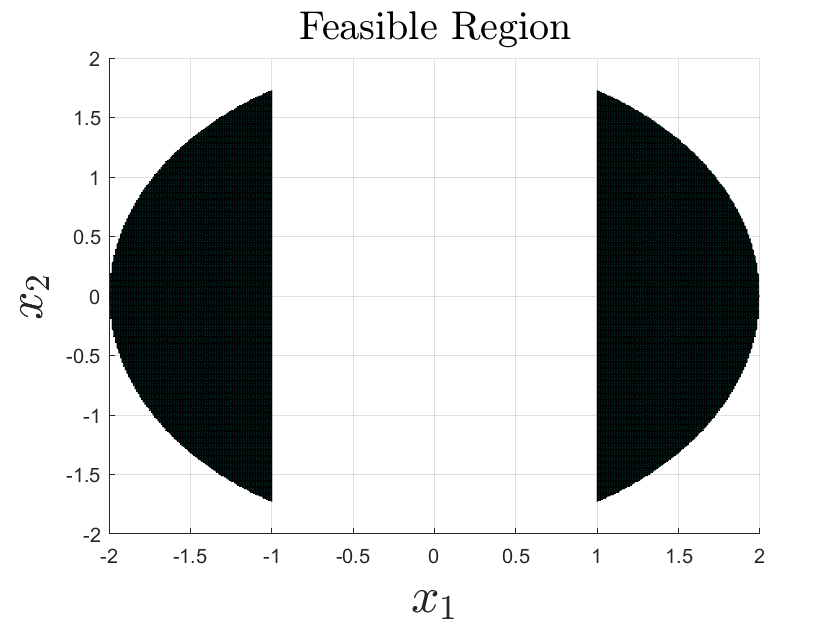
\includegraphics[scale = 0.45]{feasibleregion.png}
\end{center}
By inspection, since $f(x) = x_1$, the only local minimizer, which is also the global minimizer, is $x_* = (0,-1)^T$


\section*{Section 2.3 Problems}
\subsection*{1.} Prove that the intersection of a finite number of convex sets is also a convex set.
\newline\newline
Proof: Let $C = \{S_1, S_2, \dots, S_N\}$ be a finite collection of convex sets. Let $S_{12} = S_1 \cap S_2$ and consider the following cases:
\newline\newline
Case 1: $S_{12} = \emptyset$
\newline
Then $S_{12}$ is vacuously convex. 
\newline\newline
Case 2: $S_{12} \neq \emptyset$
\newline
Let $x, y \in S_{12}$, $0\leq \alpha \leq 1$ and consider 
\[\alpha x + (1 - \alpha)y\]
Since $x,y \in S_1$ and $S_1$ is convex, we have $\alpha x + (1 - \alpha)y \in S_1$. Similarly, $\alpha x + (1 - \alpha)y \in S_2$. Then by definition of set intersection,
\[\alpha x + (1 - \alpha)y \in S_{12}\]
So $S_{12}$ is convex by definition. 
\newline\newline
A simple induction argument shows that $S_1 \cap S_2 \cap \dots \cap S_N$ is convex. 
\newline\newline
(Note: This argument can be used to show that a countable intersection of convex sets is convex. Similarly, we may use an indexed arbitrary collection of convex sets to show that an arbitrary intersection of convex sets is also convex.)

\subsection*{2.} Let $S_1 = \{x : x_1 + x_2 \leq 1, x_1 \geq 0\}$ and $S_2 = \{x : x_1 - x_2 \geq 0, x_1 \leq 1\}$ and let $S = S_1 \cup S_2$. Prove that $S_1$ and $S_2$ are both convex sets but $S$ is not a convex set. This shows that the union of convex sets is not necessarily convex.
\newline\newline
We begin by proving that $S_1$ and $S_2$ are convex. For the remainder of this problem, let $0\leq\alpha\leq1$. To show $S_1$ is convex, let $x,y \in S_1$ and consider
\[\alpha x + (1 - \alpha)y = \begin{pmatrix}
\alpha x_1 + (1 - \alpha)y_1 \\
\alpha x_2 + (1 - \alpha)y_2 \\
\end{pmatrix}\]
Since $x,y \in S_1$, we have that $x_1, y_1 \geq 0$, and since $0 \leq \alpha \leq 1$, we have that
\[\alpha x_1 + (1 - \alpha)y_1 \geq 0\]
Now notice
\begin{align*}
    \alpha x_1 + (1 - \alpha)y_1 + \alpha x_2 + (1 - \alpha)y_2 &= \alpha(x_1 + x_2) + (1 - \alpha)(y_1 + y_2) \\
    &\leq \alpha + 1 - \alpha \\
    &= 1 \\
\end{align*}
So $\alpha x + (1 - \alpha)y \in S_1$ and thus, $S_1$ is convex by definition. Similarly, let $x,y \in S_2$ and consider 
\[\alpha x + (1 - \alpha)y = \begin{pmatrix}
    \alpha x_1 + (1 - \alpha)y_1 \\
    \alpha x_2 + (1 - \alpha)y_2 \\
\end{pmatrix}\]
Since $x,y \in S_2$, we have that $x_1, y_1 \leq 1$ and so 
\begin{align*}
    \alpha x_1+ (1 - \alpha)y_1 \leq \alpha + 1 - \alpha = 1
\end{align*}
Now notice
\begin{align*}
    [\alpha x_1 + (1 - \alpha)y_1] - [\alpha x_2 + (1 - \alpha)y_2] &= \alpha(x_1 - x_2) + (1 - \alpha)(y_1 - y_2) \\
\end{align*}
Since $x_1 - x_2 \geq 0$, $y_1 - y_2 \geq 0$, and $0 \leq \alpha \leq 1$, we have that
\[\alpha(x_1 - x_2) + (1 - \alpha)(y_1 - y_2) \geq 0\]
and so $\alpha x + (1 - \alpha)y \in S_2$ and thus, $S_2$ is convex. To show $S_1 \cup S_2$ is not convex, consider the following example:
\newline
Let $x \in S_1$, $x = \begin{pmatrix*}[r]  2\\-2\\ \end{pmatrix*}$ and $y \in S_2$, $y = \begin{pmatrix} 1\\1\\ \end{pmatrix}$ and consider
\[\alpha x + (1 - \alpha)y = \begin{pmatrix}
    \alpha + 1\\
    1 - 3\alpha\\
\end{pmatrix}\]
for $\alpha = 1/4$. Then
\[\begin{pmatrix}
    \alpha + 1\\
    1 - 3\alpha \\
\end{pmatrix}
=
\begin{pmatrix}
    5/4\\
    1/4\\
\end{pmatrix}\]
Which is not in $S_1$ or $S_2$. Then $S_1 \cup S_2$ is not convex by definition.

\subsection*{3.} Consider a feasible region $S$ defined by a set of linear constraints
\[S = \{x : Ax \leq b\}\]
Prove that $S$ is convex.
\newline\newline
Proof: Let $x, y \in S$ and let $0 \leq \alpha \leq 1$ and
\[z = \alpha x + (1- \alpha)y\]
Then
\begin{align*}
    Az &= \alpha Ax + (1 - \alpha)Ay \\
    &\leq \alpha b + (1- \alpha)b \\
    &= b\\
\end{align*}
so
\[Az \leq b\]
and thus, $z \in S$. 

\subsection*{5.} Let $f(x)$ be a function on $\mathbb{R}^n$. Prove that $f$ is both convex and concave if and only if $f(x) = c^Tx + b$ for some vector $c$ and scalar $b$.
\newline\newline
Proof: Let $f: \mathbb{R}^n \to \mathbb{R}$ be defined by $f(x) = c^Tx + b$ for $c \in \mathbb{R}^n$, $b \in \mathbb{R}$. We wish to show that $f$ is both convex and concave. From the definition of convex and concave, we must show that
\[f(\alpha x + (1 - \alpha)y) = \alpha f(x) + (1 - \alpha)f(y)\]
for $0 \leq \alpha \leq 1$. Well,
\begin{align*}
    f(\alpha x + (1 - \alpha)y) &= c^T[\alpha x + (1 - \alpha)y] + b\\
    &= \alpha c^Tx + (1 - \alpha)c^Ty + b\\
    &= \alpha c^Tx + (1 - \alpha)c^Ty + \alpha b + (1 - \alpha)b \\
    &= \alpha c^Tx + \alpha b + (1 - \alpha)c^Ty +  (1 - \alpha)b\\
    &= \alpha[c^Tx + b] + (1 - \alpha)[c^Ty + b] \\
    &= \alpha f(x) + (1 - \alpha)f(y) \\
\end{align*}
So $f$ is both convex and concave by definition. Now suppose $f$ is both convex and concave. We wish to show that $f(x) = c^Tx + b$, or in other words, affine. To begin, define $g(x) = f(x) - f(0)$. We wish to show that $g(x)$ is a linear function. We must first show that $g$ is also both convex and concave. Let $x,y \in \mathbb{R}^n$ and $0 \leq \alpha \leq 1$ and consider
\begin{align*}
    g(\alpha x + (1-\alpha)y) &= f(\alpha x + (1-\alpha)y) - f(0) \\
    &= \alpha f(x) + (1- \alpha)f(y) - \alpha f(0) + (1-\alpha)f(0) \\
    &= \alpha[f(x) - f(0)] +(1-\alpha)[f(y) - f(0)] \\
    &= \alpha g(x) + (1-\alpha)g(y) \\
\end{align*}
So $g$ is both convex and concave. Now to show $g$ is linear, we begin by showing that $g$ satisfies the homogeneity property ($g(cx) = cg(x)$ for $c \in \mathbb{R}$). Consider the following cases:
\newline\newline
Case 1: $c = 0$ or $c = 1$. This case follows trivially from definition of convexity and concavity.
\newline\newline
Case 2: $c \in (0,1)$
\newline
Notice
\begin{align*}
    g(cx) &= g(cx + (1-c)0) \\
    &= cg(x) + (1-c)g(0) \\
    &= cg(x) \\
\end{align*}
\newline\newline
Case 3: $c \in (1, \infty)$
\newline
Notice 
\begin{align*}
    g(x) &= g\left(\frac{1}{c}cx + (1 - 1/c)0\right) \\
    &= \frac{1}{c}g(cx) + (1 - 1/c)g(0) \\
    &= \frac{1}{c}g(cx) \\
\end{align*}
And multiplying both sides by $c$, we have
\[g(cx) = cg(x)\]
\newline\newline
Case 3: $c = -1$ (This case, along with the previous 2 cases will verify homogeneity holds for $c \in \mathbb{R}$)
\newline
Notice
\begin{align*}
    g(x) &= g(2x - x) \\
    &= 2g(x) + g(-x) \\
    -g(x) &= g(-x) \\
\end{align*}
So homogeneity holds. Now we must verify linearity holds. Let $x, y \in \mathbb{R}^n$ and consider $g(x+y)$. Notice the following:
\begin{align*}
    g(x+ y) &= g(2/2x + 2/2y) \\
    &= 1/2g(2x) + 1/2g(2y) \\
    &= 2/2g(x) + 2/2g(y) \\
    &= g(x) + g(y) \\
\end{align*}
So linearity holds. Then by definition of linear functions, $g$ is linear. Then $g(x) + f(0) = f(x)$ is affine by definition. Recall that the general form of an affine function takes the following form:
\[f(x) = c^Tx + b\]
for $c \in \mathbb{R}^n$, $b\in \mathbb{R}$, which is what we sought to show.


\subsection*{20.} Determine if 
\[f(x_1,x_2) = 2x_1^2 - 3x_1x_2 + 5x_2^2 - 2x_1 + 6x_2\]
is convex, concave, both, or neither for $x \in \mathbb{R}^2$.
\newline\newline
To determine if $f(x)$ is convex, concave, both, or neither, we must inspect the Hessian of $f$. Well, the gradient of $f$ is as follows:
\[\nabla f(x) = \begin{pmatrix}
    4x_1 - 3x_2 - 2\\
    -3x_1 + 10x_2 + 6\\
\end{pmatrix}\]
and so the Hessian is
\[\nabla^2f(x) = \begin{pmatrix}
    4 & -3 \\
    -3 & 10\\
\end{pmatrix}\]
Row reducing as in Gaussian elimination, it is easily shown that the row echelon form of the Hessian is 
\[\begin{pmatrix}
    4 & -3\\
    0 & 31/4\\
\end{pmatrix}\]
Since the row echelon form of $\nabla^2f(x)$ has strictly positive pivots, we have that $\nabla^2f(x)$ is positive definite, so $f(x)$ is strictly convex.

\section*{Section 2.4 Problems}
\subsection*{2.} Find all descent directions for the linear function $f(x) = x_1 - 2x_2 + 3x_3$. Does your answer depend on the value of $x$?
\newline\newline
Recall that the direction of greatest descent is given by the negative gradient:
\[-\nabla f(x) = \begin{pmatrix*}[r]
    -1\\
    2\\
    -3\\
\end{pmatrix*}\]
And notice that $p$ is a descent direction for $f(x)$ provided $p^T\nabla f(x) > 0$. That is, $p$ is a descent direction provided $-p_1 + 2p_2 - 3p_3 > 0$. Let $D$ be the set of descent directions for $f(x)$. Then
\[D = \{p \in \mathbb{R}^3 \: | \: -p_1 + 2p_2 - 3p_3 > 0\}\]

\section*{Section 2.6 Problems}
\subsection*{1.} Find the first four terms of the Taylor series for 
\[f(x) = \log(1 + x)\]
about the point $x_0 = 0$. Evaluate the series for $p = 0.1$ and $p = 0.01$ and compare with the value of $f(x_0 + p)$. Derive the remainder form of the Taylor series using five terms (the four terms you already derived plus a remainder term). Derive a bound on the accuracy of the four-term series. Compare the bound you derived with the actual errors for $p = 0.1$ and $p = 0.01$.
\newline\newline
Recall the general form of a Taylor series of a function centered at $x = x_0$:
\[f(x) = \sum_{k=0}^{\infty}\frac{f^{(k)}(x_0)}{k!}(x-x_0)^k\]
where $f^{(0)}(x_0) = f(x_0)$. Using this and the fact that the general form for the $n^{\text{th}}$ derivative of $\log(1 + x)$ is $\frac{d^n}{dx^n}\log(1 + x) = \frac{(-1)^{n-1}(n-1)!}{(1 + x)^n}$, we find the following fourth order expansion:
\[\log(1 + x) \approx p(x) = x - \frac{x^2}{2} + \frac{x^3}{3} - \frac{x^4}{4}\]
Evaluating this series at $p = 0.1$ and $p = 0.01$, we find the following values:
\begin{align*}
    p(0.1) &\approx 0.0953083 \\
    \log(1 + 0.1) &\approx 0.0953102 \\
\end{align*}
With an associated error of 
\[|p(0.1) - \log(1.1)| = 1.8465 \times 10^{-6}\]
\begin{align*}
    p(0.01) &\approx 0.009950330833 \\
    \log(1 + 0.01) &\approx 0.009950330835 \\
\end{align*}
With an associated error of
\[|p(0.01) - \log(1.01)| = 1.983476 \times 10^{-11}\]
From Taylor's Theorem, the error term of the fourth order expansion takes the following form:
\[R_4(x) = \frac{x^5}{5(1 + \xi)^5}\]
where $\xi$ is between 0 and $x$. For $x \geq 0$, we have that 
\begin{align*}
    |R_4(x)| = \left|\frac{x^5}{5(1+\xi)^5}\right| \leq \frac{x^5}{5} \\
\end{align*}
Then an error bound for $p = 0.1$ is given by
\[|R_4(0.1)| \leq \frac{0.1^5}{5} = 2 \times 10^{-6}\]
Notice that $|p(0.1) - \log(1.1)|$ is within this error bound! Now, our error bound for $p = 0.01$ is given by
\[|R_4(0.01)| \leq \frac{0.01^5}{5} = 2 \times 10^{-11}\]
Notice that $|p(0.01) - \log(1.01)|$ is also within this error bound! Math works!


\subsection*{4.} Find the first three terms of the Taylor series for 
\[f(x_1, x_2) = 3x_1^4 - 2x_1^3x_2 - 4x_1^2x_2^2 + 5x_1x_2^3 + 2x_2^4\]
at the point
\[x_0 = (1, -1)^T.\]
From Taylor's Theorem, the first three terms of a multivariate expansion take the following form:
\[f(x) \approx f(x_0) + (x - x_0)^T\nabla f(x_0) + (x - x_0)^T\nabla^2f(x_0)(x - x_0)\]
Notice for our function,
\begin{align*}
    \nabla f(x) = \begin{pmatrix}
        12x_1^4 - 6x_1^2x_2 - 8x_1x_2^2 + 5x_3 \\
        -2x_1^3 - 8x_1^2x_2 + 15x_1x_2^2 + 8x_2^3 \\
    \end{pmatrix}
\end{align*}
and 
\begin{align*}
    \nabla^2f(x) = \begin{pmatrix}
        36x_1^2 - 12x_1x_2 - 8x_2^2 & -6x_1^2 - 16x_1x_2 + 15x_2^2 \\
        -6x_1^2 - 16x_1x_2 + 15x_2^2 & -8x_1^2 + 30x_1x_2 + 24x_2^2 \\
    \end{pmatrix}
\end{align*}
And at $x = x_0$, we have
\[f(x_0) = -2\]

\begin{align*}
    \nabla f(x_0) = \begin{pmatrix}
        5 \\
        13 \\
    \end{pmatrix}
\end{align*}
and
\begin{align*}
    \nabla^2f(x_0) = \begin{pmatrix}
        40 & 25 \\
        25 & -14 \\
    \end{pmatrix}
\end{align*}
So 
\begin{align*}
    f(x) &\approx -2 + (x_1 - 1, x_2 + 1)\begin{pmatrix}
        5 \\
        13 \\
    \end{pmatrix}
    + (x_1 - 1, x_2 + 1)\begin{pmatrix}
        40 & 25 \\
        25 & -14 \\
    \end{pmatrix}
    \begin{pmatrix}
        x_1 - 1 \\
        x_2 + 1 \\
    \end{pmatrix} \\
    &= 40x_1^2 - 14x_2^2 + 50x_1x_2 - 25x_1 - 65x_2 - 18 \\
\end{align*}

\subsection*{6.} Prove that if $p^T\nabla f(x_k) < 0$, then $f(x_k + \epsilon p) < f(x_k)$ for $\epsilon > 0$ sufficiently small. Hint: expand $f(x_k + \epsilon p)$ in a Taylor series about the point $x_k$ and look at $f(x_k + \epsilon p) - f(x_k)$.
\newline\newline
Proof: Let $f$ be continuously differentiable and let $p^T\nabla f(x_k) < 0$ and consider $f(x_k + \epsilon p)$ for $\epsilon > 0$. We wish to show $f(x_k + \epsilon p) < f(x_k)$ for $\epsilon$ sufficiently small. Taylor expanding $f(x_k + \epsilon p)$, we find
\begin{align*}
    f(x_k + \epsilon p) &= f(x_k) + \epsilon p^T\nabla f(x_k + tp) \\
\end{align*}
For some $t \in (0, \epsilon)$. Then by continuity of $\nabla f$ and the fact that $p^T\nabla f(x_k) < 0$, we have for some $\epsilon > 0$, $p^T\nabla f(x_k + \epsilon p) < 0$, and since $t \in (0, \epsilon)$, we have $p^T\nabla f(x_k + tp) < 0$ and so
\begin{align*}
    f(x_k + \epsilon p) - f(x_k) &= \epsilon p^T\nabla f(x_k + tp) \\
    f(x_k + \epsilon p) - f(x_k) &< 0 \\
    f(x_k + \epsilon p) &< f(x_k) \\
\end{align*}
which is what we sought to show.

\subsection*{8.} Let $f$ be a real-valued function of $n$ variables $x$ with continuous second derivatives. Use the result of the previous problem to prove that $f$ is convex on the convex set $S$ if $\nabla^2f(x)$ is positive semidefinite for all $x \in S$.
\newline\newline
Proof: Let $f \: : \: \mathbb{R}^n \to \mathbb{R}$ have continuous second derivatives and suppose that $\nabla^2f(x)$ is positive semi definite for all $x \in S$. By Taylor's theorem, we have
\begin{align*}
    f(y) &= f(x) + \nabla f(x)^T(y-x) + (y-x)^T\nabla^2f(\xi)(y-x) \\
\end{align*}
for some $\xi\in \mathbb{R}^n$ between $x$ and $y$. Since $\nabla^2f(x)$ is positive semi definite, we have that
\begin{align*}
    f(y) &\geq f(x) + \nabla f(x)^T(y-x) \\
\end{align*}
which, by 2.6.7, gives us that $f$ is convex on $S$.
\end{document}
